\documentclass[12pt]{article}
\usepackage{tikz}
\usetikzlibrary{decorations.pathmorphing}
\usepackage{amsmath}
\usepackage{amssymb}
\usepackage{xcolor}
\usepackage{geometry}
\geometry{a4paper, margin=1in}

% 定义原代码中使用的颜色
\definecolor{blue3}{RGB}{0,0,205}
\definecolor{lightgray2}{RGB}{211,211,211}
% 定义原代码中使用的 \mb 命令
\newcommand{\mb}[1]{\mathbf{#1}}

\begin{document}

\section*{Diagram 1: Original Bubble Diagram}
\begin{figure}[ht] 
    \centering 
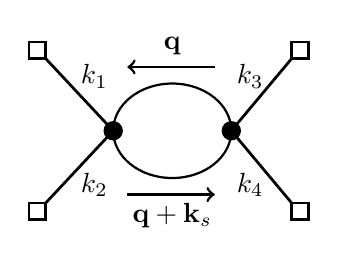
\begin{tikzpicture}[baseline={([yshift=-.5ex]current bounding box.center)}, line width=1. pt, scale=3.] 
    \draw[black, thick] (0.25,0) ellipse (0.25 and 0.20); 
    \draw[black] (0, 0) -- (-0.285, 0.305); 
    \draw[black] (0, 0) -- (-0.285, -0.305); 
    \node[draw, rectangle, minimum width=6.0pt, minimum height=6.0pt, inner sep=0pt, anchor=south east] at (-0.28,0.3) {}; 
    \node[draw, rectangle, minimum width=6.0pt, minimum height=6.0pt, inner sep=0pt, anchor=north east] at (-0.28,-0.3) {}; 
    \draw[black] (0.5, 0) -- (0.755, 0.305); 
    \draw[black] (0.5, 0) -- (0.755, -0.305); 
    \draw[draw=black, fill=black] (0, 0) circle (.035cm); 
    \draw[draw=black, fill=black] (0.5, 0) circle (.035cm); 
    \node[draw, rectangle, minimum width=6.0pt, minimum height=6.0pt, inner sep=0pt, anchor=south west] at (0.75,0.3) {}; 
    \node[draw, rectangle, minimum width=6.0pt, minimum height=6.0pt, inner sep=0pt, anchor=north west] at (0.75,-0.3) {}; 
    \node at (-0.08, 0.23) {$k_1$}; 
    \node at (-0.08, -0.23) {$k_2$}; 
    \node at (0.58, 0.23) {$k_3$}; 
    \node at (0.58, -0.23) {$k_4$}; 
    \node at (0.25,0.36){$\mb q$}; 
    \node at (0.25,-0.36){$\mb q+\mb k_s$}; 
    \draw[<-,black] (0.06,0.27)--(0.43,0.27); 
    \draw[->,black] (0.06,-0.27)--(0.43,-0.27); 
\end{tikzpicture} 
    \caption{SK diagrams for four-point correlators with bubble topology. All loop and external lines are black. The \(\Box\) vertices lie on the future boundary, and the \textcolor{black}{$\bullet$} vertices denote bulk insertions on the two Schwinger-Keldysh contours, with \(+\) and \(-\) corresponding to the time-ordered and anti-time-ordered branches, respectively. Contributions from all SK branches are summed.\label{fig_bubble}} 
\end{figure} 

\vspace{1cm}

\section*{Diagram 2: Bubble with Massless (Photon) Line}
\begin{figure}[ht] 
    \centering 
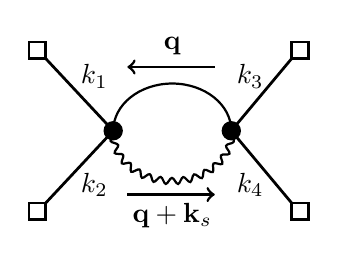
\begin{tikzpicture}[baseline={([yshift=-.5ex]current bounding box.center)}, line width=1. pt, scale=3.] 
    % 上半部分保留为黑色线条
    \draw[black, thick] (0.5,0) arc (0:180:0.25 and 0.20); 
    % 下半部分替换为表示无质量的光子传播子波浪线 (黑色)
    \draw[decorate, decoration={snake, amplitude=0.4mm, segment length=1.5mm}, thick, black] (0,0) arc (180:360:0.25 and 0.20);
    
    \draw[black] (0, 0) -- (-0.285, 0.305); 
    \draw[black] (0, 0) -- (-0.285, -0.305); 
    \node[draw, rectangle, minimum width=6.0pt, minimum height=6.0pt, inner sep=0pt, anchor=south east] at (-0.28,0.3) {}; 
    \node[draw, rectangle, minimum width=6.0pt, minimum height=6.0pt, inner sep=0pt, anchor=north east] at (-0.28,-0.3) {}; 
    \draw[black] (0.5, 0) -- (0.755, 0.305); 
    \draw[black] (0.5, 0) -- (0.755, -0.305); 
    \draw[draw=black, fill=black] (0, 0) circle (.035cm); 
    \draw[draw=black, fill=black] (0.5, 0) circle (.035cm); 
    \node[draw, rectangle, minimum width=6.0pt, minimum height=6.0pt, inner sep=0pt, anchor=south west] at (0.75,0.3) {}; 
    \node[draw, rectangle, minimum width=6.0pt, minimum height=6.0pt, inner sep=0pt, anchor=north west] at (0.75,-0.3) {}; 
    \node at (-0.08, 0.23) {$k_1$}; 
    \node at (-0.08, -0.23) {$k_2$}; 
    \node at (0.58, 0.23) {$k_3$}; 
    \node at (0.58, -0.23) {$k_4$}; 
    \node at (0.25,0.36){$\mb q$}; 
    \node at (0.25,-0.36){$\mb q+\mb k_s$}; 
    \draw[<-,black] (0.06,0.27)--(0.43,0.27); 
    \draw[->,black] (0.06,-0.27)--(0.43,-0.27); 
\end{tikzpicture} 
    \caption{Bubble diagram with the bottom propagator replaced by a massless (photon-like) line.} 
\end{figure} 

\vspace{1cm}

\section*{Diagram 3: Contracted Tadpole Diagram}
\begin{figure}[ht] 
    \centering 
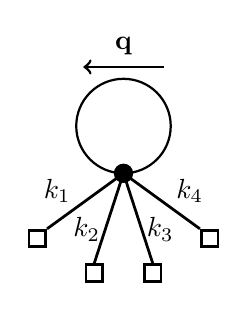
\begin{tikzpicture}[baseline={([yshift=-.5ex]current bounding box.center)}, line width=1. pt, scale=3.] 
    
    % 上方的圈保留 (tadpole loop)
    \draw[black, thick] (0, 0.2) circle (0.20);
    
    % 四个外线放置在下半平面，五等分 (角度: 216, 252, 288, 324)
    % 半径设为 0.4
    \draw[black] (0, 0) -- (216:0.4); 
    \draw[black] (0, 0) -- (252:0.4); 
    \draw[black] (0, 0) -- (288:0.4); 
    \draw[black] (0, 0) -- (324:0.4); 

    % 收缩后的单一顶点，位于 (0, 0) (放在最后绘制，覆盖在线上方)
    \draw[draw=black, fill=black] (0, 0) circle (.035cm); 

    % 外线端点加方框
    \node[draw, rectangle, minimum width=6.0pt, minimum height=6.0pt, inner sep=0pt, anchor=north east] at (216:0.4) {}; 
    \node[draw, rectangle, minimum width=6.0pt, minimum height=6.0pt, inner sep=0pt, anchor=north] at (252:0.4) {}; 
    \node[draw, rectangle, minimum width=6.0pt, minimum height=6.0pt, inner sep=0pt, anchor=north] at (288:0.4) {}; 
    \node[draw, rectangle, minimum width=6.0pt, minimum height=6.0pt, inner sep=0pt, anchor=north west] at (324:0.4) {}; 
    
    % 外线动量标签
    \node at (216:0.25) [above left=-2pt] {$k_1$}; 
    \node at (252:0.25) [left=-2pt] {$k_2$}; 
    \node at (288:0.25) [right=-2pt] {$k_3$}; 
    \node at (324:0.25) [above right=-2pt] {$k_4$}; 
    
    % 圈上动量及箭头
    \node at (0, 0.54) {$\mb q$}; 
    \draw[<-,black] (-0.17, 0.45) -- (0.17, 0.45); 
\end{tikzpicture} 
    \caption{Tadpole diagram obtained by contracting the bottom loop propagator. All external lines are arranged in the lower half-plane.} 
\end{figure}  

\vspace{1cm}

\section*{Diagram 4: Original Bubble Diagram (Gray Vertices)}
\begin{figure}[ht] 
    \centering 
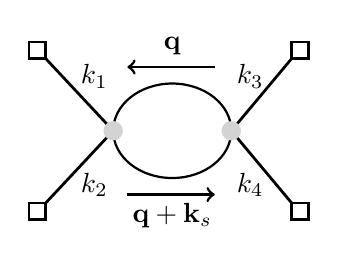
\begin{tikzpicture}[baseline={([yshift=-.5ex]current bounding box.center)}, line width=1. pt, scale=3.] 
    \draw[black, thick] (0.25,0) ellipse (0.25 and 0.20); 
    \draw[black] (0, 0) -- (-0.285, 0.305); 
    \draw[black] (0, 0) -- (-0.285, -0.305); 
    \node[draw, rectangle, minimum width=6.0pt, minimum height=6.0pt, inner sep=0pt, anchor=south east] at (-0.28,0.3) {}; 
    \node[draw, rectangle, minimum width=6.0pt, minimum height=6.0pt, inner sep=0pt, anchor=north east] at (-0.28,-0.3) {}; 
    \draw[black] (0.5, 0) -- (0.755, 0.305); 
    \draw[black] (0.5, 0) -- (0.755, -0.305); 
    \draw[draw=lightgray2, fill=lightgray2] (0, 0) circle (.035cm); 
    \draw[draw=lightgray2, fill=lightgray2] (0.5, 0) circle (.035cm); 
    \node[draw, rectangle, minimum width=6.0pt, minimum height=6.0pt, inner sep=0pt, anchor=south west] at (0.75,0.3) {}; 
    \node[draw, rectangle, minimum width=6.0pt, minimum height=6.0pt, inner sep=0pt, anchor=north west] at (0.75,-0.3) {}; 
    \node at (-0.08, 0.23) {$k_1$}; 
    \node at (-0.08, -0.23) {$k_2$}; 
    \node at (0.58, 0.23) {$k_3$}; 
    \node at (0.58, -0.23) {$k_4$}; 
    \node at (0.25,0.36){$\mb q$}; 
    \node at (0.25,-0.36){$\mb q+\mb k_s$}; 
    \draw[<-,black] (0.06,0.27)--(0.43,0.27); 
    \draw[->,black] (0.06,-0.27)--(0.43,-0.27); 
\end{tikzpicture} 
    \caption{SK diagrams for four-point correlators with bubble topology. All loop and external lines are black. The \(\Box\) vertices lie on the future boundary, and the \textcolor{lightgray2}{$\bullet$} vertices denote bulk insertions on the two Schwinger-Keldysh contours, with \(+\) and \(-\) corresponding to the time-ordered and anti-time-ordered branches, respectively. Contributions from all SK branches are summed.} 
\end{figure} 

\vspace{1cm}

\section*{Diagram 5: Original Bubble Diagram (One Black, One White Vertex)}
\begin{figure}[ht] 
    \centering 
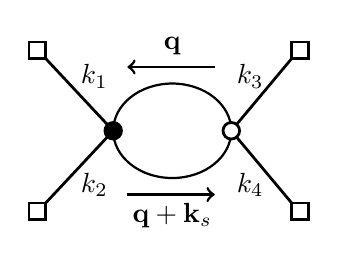
\begin{tikzpicture}[baseline={([yshift=-.5ex]current bounding box.center)}, line width=1. pt, scale=3.] 
    \draw[black, thick] (0.25,0) ellipse (0.25 and 0.20); 
    \draw[black] (0, 0) -- (-0.285, 0.305); 
    \draw[black] (0, 0) -- (-0.285, -0.305); 
    \node[draw, rectangle, minimum width=6.0pt, minimum height=6.0pt, inner sep=0pt, anchor=south east] at (-0.28,0.3) {}; 
    \node[draw, rectangle, minimum width=6.0pt, minimum height=6.0pt, inner sep=0pt, anchor=north east] at (-0.28,-0.3) {}; 
    \draw[black] (0.5, 0) -- (0.755, 0.305); 
    \draw[black] (0.5, 0) -- (0.755, -0.305); 
    \draw[draw=black, fill=black] (0, 0) circle (.035cm); 
    \draw[draw=black, fill=white] (0.5, 0) circle (.035cm); 
    \node[draw, rectangle, minimum width=6.0pt, minimum height=6.0pt, inner sep=0pt, anchor=south west] at (0.75,0.3) {}; 
    \node[draw, rectangle, minimum width=6.0pt, minimum height=6.0pt, inner sep=0pt, anchor=north west] at (0.75,-0.3) {}; 
    \node at (-0.08, 0.23) {$k_1$}; 
    \node at (-0.08, -0.23) {$k_2$}; 
    \node at (0.58, 0.23) {$k_3$}; 
    \node at (0.58, -0.23) {$k_4$}; 
    \node at (0.25,0.36){$\mb q$}; 
    \node at (0.25,-0.36){$\mb q+\mb k_s$}; 
    \draw[<-,black] (0.06,0.27)--(0.43,0.27); 
    \draw[->,black] (0.06,-0.27)--(0.43,-0.27); 
\end{tikzpicture} 
    \caption{SK diagrams for four-point correlators with bubble topology. The \(\Box\) vertices lie on the future boundary, and the \textcolor{black}{$\bullet$} and $\circ$ vertices denote bulk insertions on the two Schwinger-Keldysh contours.} 
\end{figure} 

\end{document}